\message{ !name(thesis.tex)}\documentclass[twoside,11pt]{article}

% Any additional packages needed should be included after jmlr2e.
% Note that jmlr2e.sty includes epsfig, amssymb, natbib and graphicx,
% and defines many common macros, such as 'proof' and 'example'.
%
% It also sets the bibliographystyle to plainnat; for more information on
% natbib citation styles, see the natbib documentation, a copy of which
% is archived at http://www.jmlr.org/format/natbib.pdf

\usepackage{jmlr2e}
\usepackage{listings}
\usepackage{graphicx}
\usepackage{subfigure}
\usepackage[margin=0.75in]{geometry}
\usepackage{courier}
\usepackage{color}
\usepackage{listings}
\usepackage{algorithm}
\usepackage{algorithmic}
\usepackage{multirow}
\usepackage{rotating}
\usepackage{enumerate}

\definecolor{dkgreen}{rgb}{0,0.6,0}
\definecolor{gray}{rgb}{0.5,0.5,0.5}

\begin{document}

\message{ !name(thesis.tex) !offset(571) }
\begin{figure}
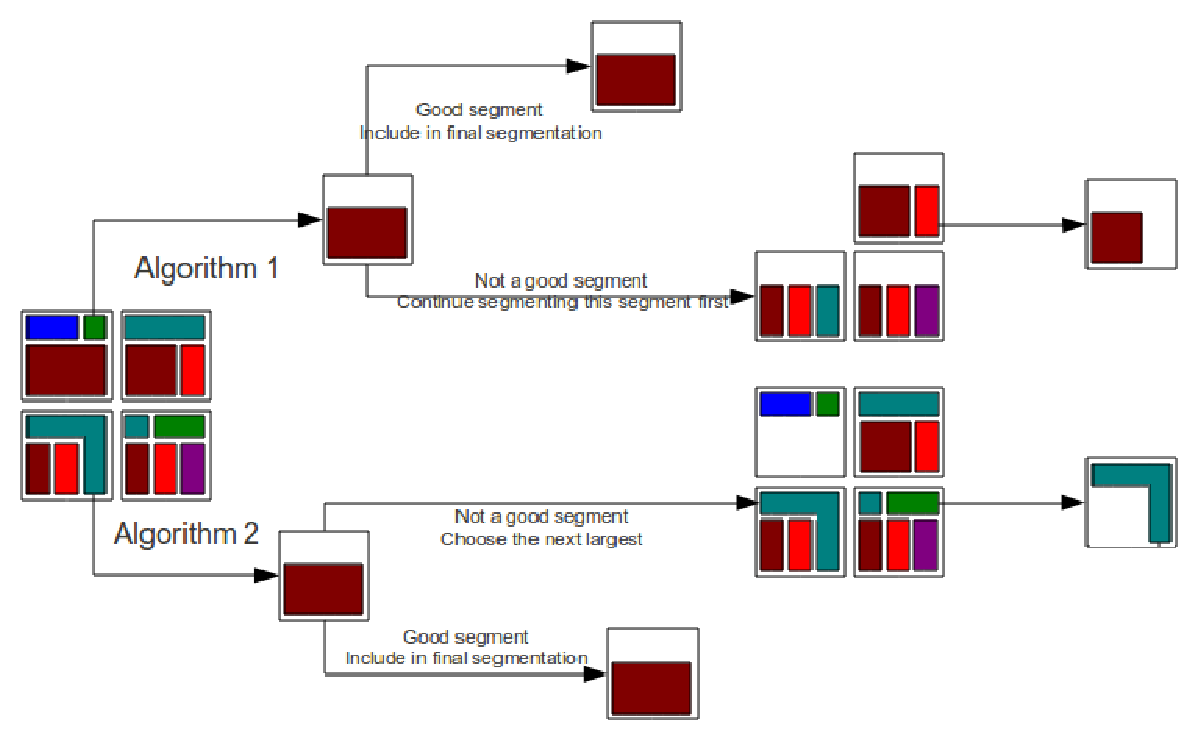
\includegraphics[scale =.8]{./Figures/mixsegs.eps}
\centering
\caption{2 Steps in mixing 4 different segmentations with the two algorithms
segments are represented by large colorful squares to better clarify the idea.}
\label{fig:mixsegsalgo}
\end{figure}
\message{ !name(thesis.tex) !offset(1710) }

\end{document}
